\documentclass[mathserif, 10pt, dvipsnames]{beamer}
\usepackage[utf8]{inputenc}
\usepackage{amsmath, amsfonts}
\usepackage{appendixnumberbeamer}



\title[Using ML techniques in phenomenological studies in flavour physics]{Using Machine Learning techniques in\\ phenomenological studies in flavour physics}
\subtitle{Jorge Alda,\\ Universidad de Zaragoza/CAPA \hspace{4em} \texttt{jalda@unizar.es} }
\author[Jorge Alda]{Based on \textbf{JA}, J. Guasch, S. Peñaranda \\
arXiv:2109.07405 [hep-ph]}

\date[CERN Workshop]{5th Inter-experiment Machine Learning Workshop\\ 9-13th May 2022}



\usetheme{Zaragoza}
\usecolortheme{Unizar}
\titlepagelogoA{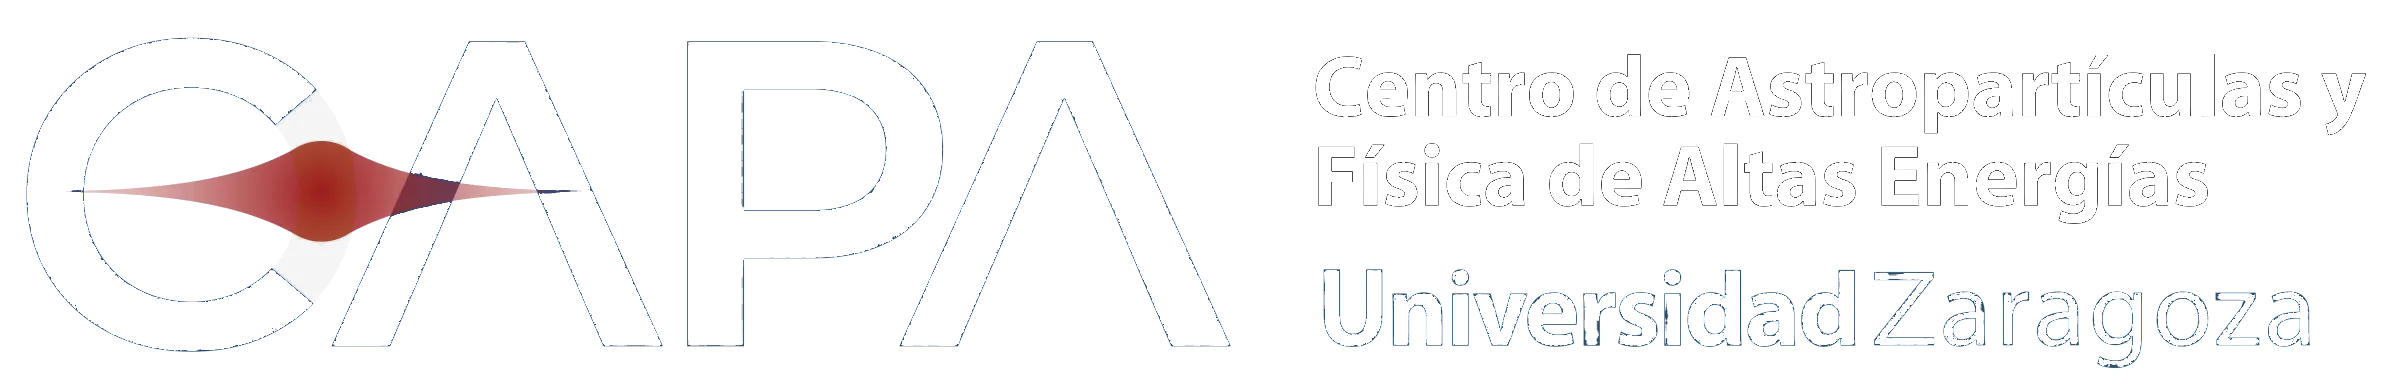
\includegraphics[width=6cm]{logos/CAPA.png}}
\titlepagelogoB{
\includegraphics[width=4cm]{logos/dftuz2.png}}


\newcommand\colorcite[1]{{\scriptsize\color{blue}#1}}

\begin{document}
\begin{frame}[noframenumbering,plain]

\titlepage

\end{frame}

\begin{frame}\frametitle{Problem}
\begin{itemize}
\item We study $R_{K^{(*)}}$ and $R_{D^{(*)}}$ anomalies affecting $B$ meson decays
    \item using Effective Field Theory at $\Lambda = 1\,\mathrm{TeV}$.
$$\mathcal{L}_\mathrm{EFT} = \mathcal{L}_\mathrm{SM} + \frac{1}{\Lambda^2} {\color{red}C} {\color{OliveGreen}\lambda^\ell_{ij}} {\color{blue}\lambda^q_{kl}}\left[ (\bar{\ell}_i \gamma_\mu \ell_j)(\bar{q}_k \gamma^\mu  q_l) + (\bar{\ell}_i \gamma_\mu \tau^I \ell_j)(\bar{q}_k \gamma^\mu \tau^I q_l) \right].$$
\item Global fits with 5 parameters ({\color{red}$C$}, {\color{OliveGreen}$\alpha^\ell$}, {\color{OliveGreen}$\beta^\ell$}, {\color{blue}$\alpha^q$}, {\color{blue}$\beta^q$}), log-likelihood function contains 471 physical observables.
\end{itemize}
\begin{columns}[onlytextwidth]
    \begin{column}{0.7\textwidth}
        \begin{itemize}
            \item Non-linear relations $\Longrightarrow$ equi-probability regions are not elliptical $\Longrightarrow$ we can not use Hessian approximation for the log-likelihood.
        \end{itemize}
    \end{column}
    \begin{column}{0.25\textwidth}
        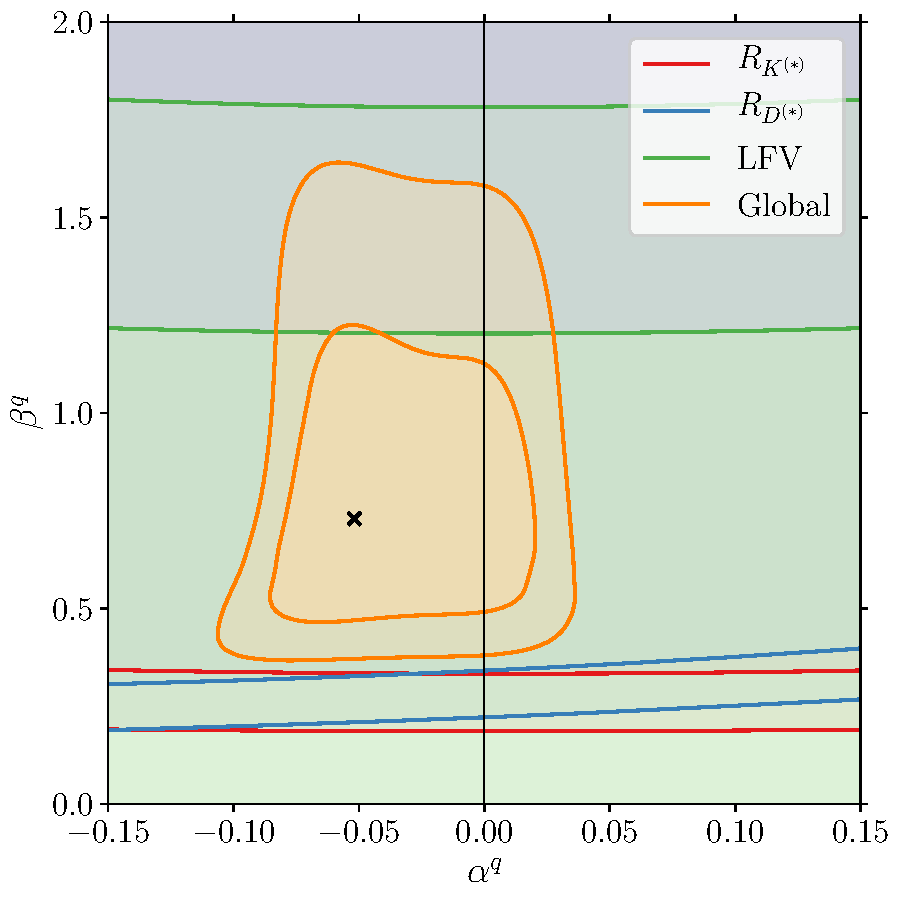
\includegraphics[width=\textwidth]{figures/alphabeta_q.pdf}
    \end{column}
\end{columns}
\end{frame}

\begin{frame}\frametitle{Machine Learning training}

    \textbf{Solution:} We create an approximation of the log-likelihood function using the \texttt{xgboost} model (regression tree).

    \begin{columns}
        \begin{column}{0.5\textwidth}
            Data sample consisting of
            \begin{itemize}
                \item 5000 points re-used from likelihood plots.
                \item 5000 random points.
                \item Split in 75\% training set, 25\% validation set.
                \item Learning rate 0.05, 1000 estimators, early stopping at 5 rounds.
            \end{itemize}
            Results of the training:
            \begin{itemize}
                \item Pearson regression coefficient $r=0.971$.
                \item Mean Absolute Error $0.655$.
            \end{itemize}
        \end{column}
        \begin{column}{0.5\textwidth}
            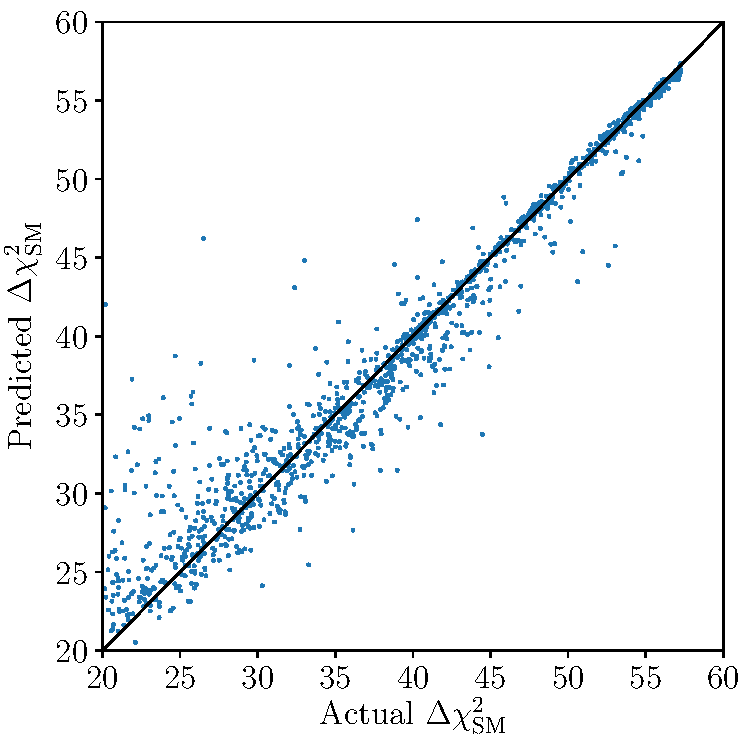
\includegraphics[width=\columnwidth]{figures/regression_xgb.pdf}
        \end{column}
    \end{columns}

\end{frame}

\begin{frame}\frametitle{Machine Learning Montecarlo}
    \begin{columns}
        \begin{column}{0.5\textwidth}
            We want to generate a sample of points distributed according to the $\chi^2$ of the fit.

            We generate random points, that are accepted if
            $$\log \tilde{L}(\vec{C}) = \log L_\mathrm{bf} + \log u\,,$$
            with $u$ a random number from the uniform distribution in $[0,1)$. % chktex 9
        \end{column}
        \begin{column}{0.5\textwidth}
            {\small Montecarlo points generated using the
                Machine Learning algorithm:}\\[0.2em]
            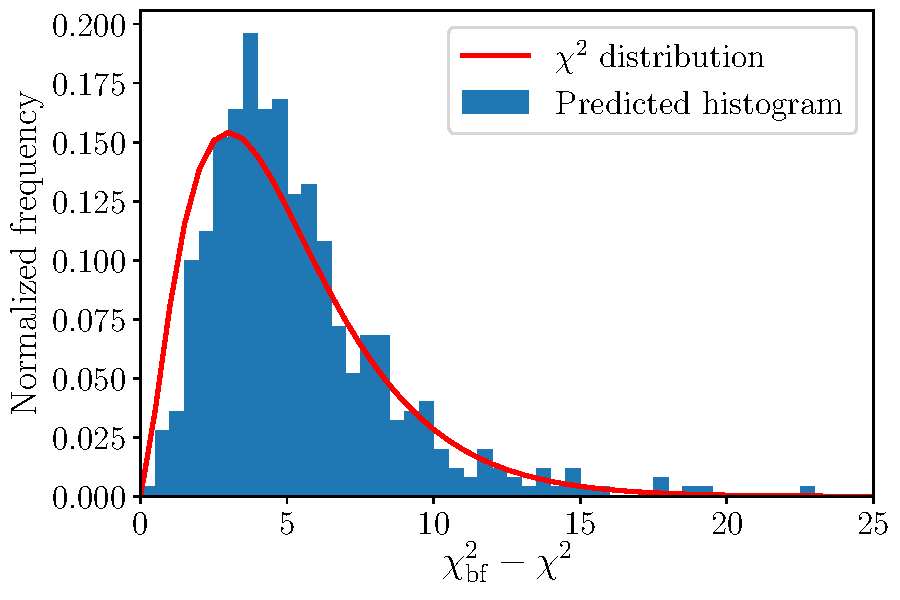
\includegraphics[width=\columnwidth]{figures/hist_xgb.pdf}
        \end{column}
    \end{columns}

    ~

    We use the trained model $\log\tilde{L}(\vec{C})$ to compute an approximation of the likelihood function.

\end{frame}

\begin{frame}\frametitle{SHAP values}

    We calculate \texttt{SHAP} values in the Montecarlo sample to examine the importance of each parameter in the \texttt{xgboost} predictions.

    \vspace{0.5cm}

    The mixing \(\beta^q\) to the second quark generation ($b\to s$ and $b \to c$) and $\alpha^\ell$ to the first lepton generation (explains $R_{K^{(*)}}$) are in general the most important features.
    \begin{center}
        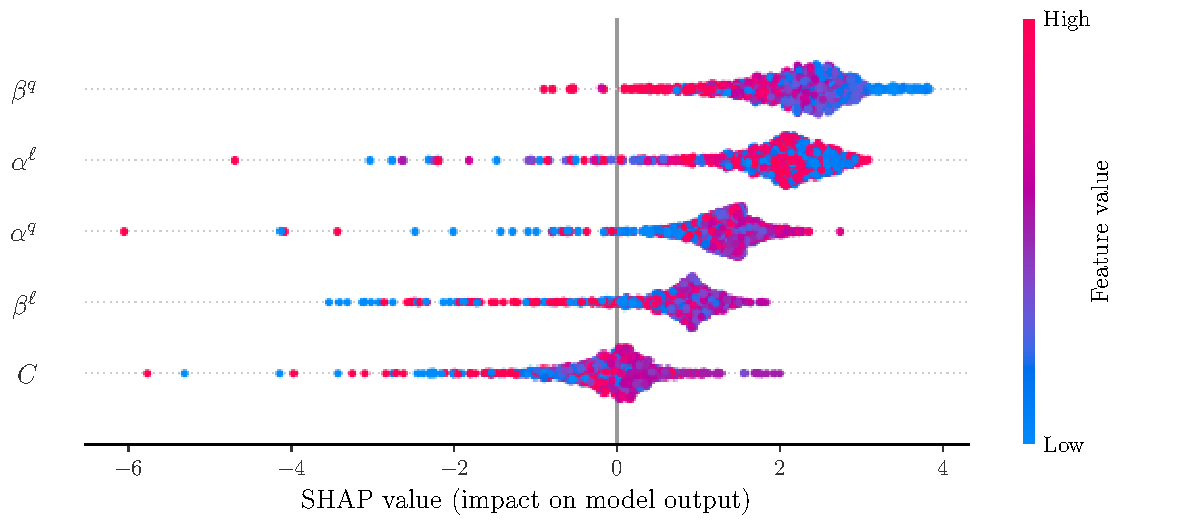
\includegraphics[width=0.8\textwidth]{figures/SHAP_summary.pdf}
    \end{center}
\end{frame}

\begin{frame}\frametitle{SHAP values and likelihood}
    \texttt{SHAP} importances reproduce the dependence of the $-\log L$:
    \begin{center}
        {\small \qquad\qquad$C\qquad\qquad\qquad\qquad \alpha^\ell \qquad\qquad\qquad\qquad\qquad\beta^q\qquad$} \\
        \rotatebox{90}{\small $\qquad\Delta \log L$}
        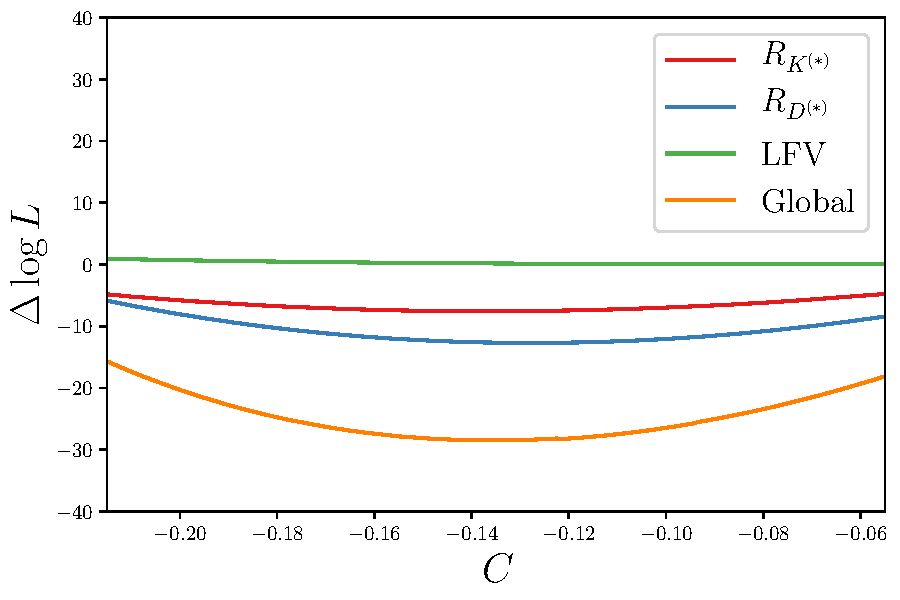
\includegraphics[width=0.30\textwidth]{figures/evoplot_C.pdf}
        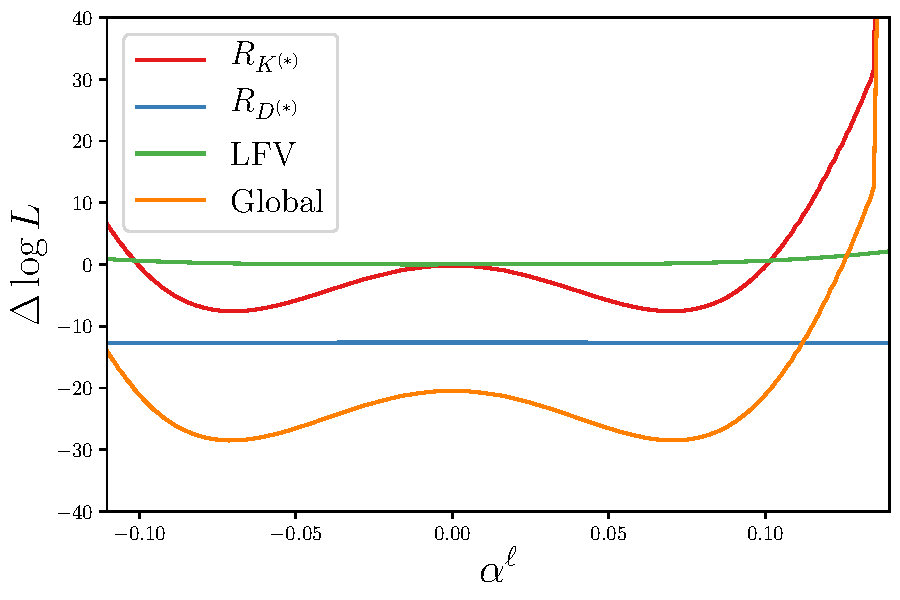
\includegraphics[width=0.30\textwidth]{figures/evoplot_alphal.pdf}
        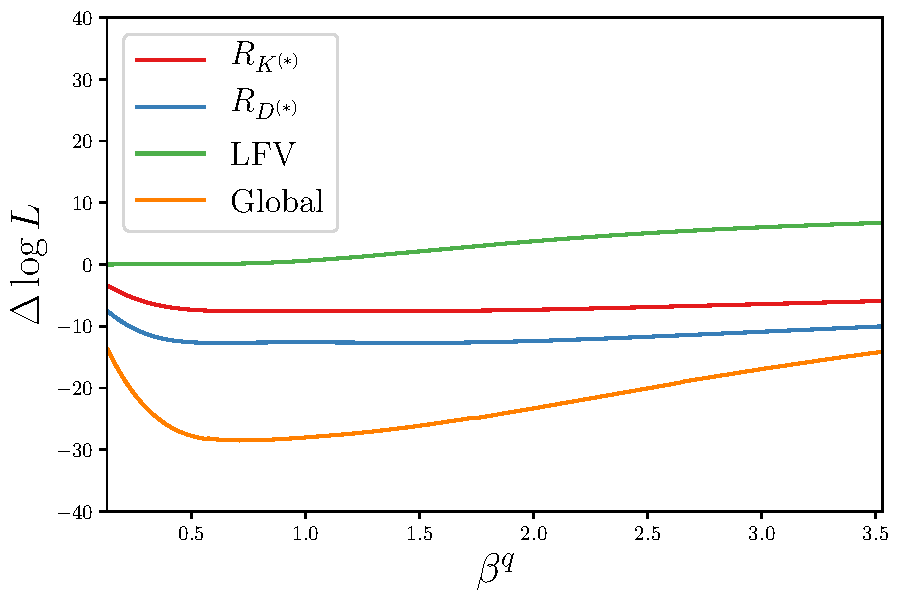
\includegraphics[width=0.30\textwidth]{figures/evoplot_betaq.pdf}
    \end{center}
    \begin{center}
        \rotatebox{90}{\small $\qquad\qquad\mathrm{SHAP}$}
        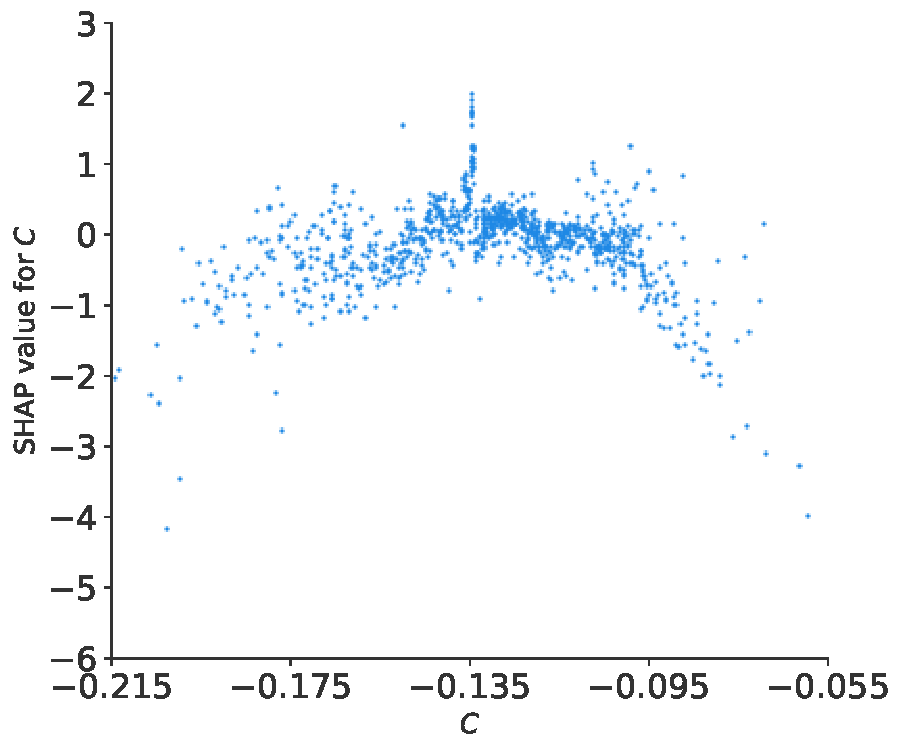
\includegraphics[width=0.30\textwidth]{figures/SHAP_C.pdf}
        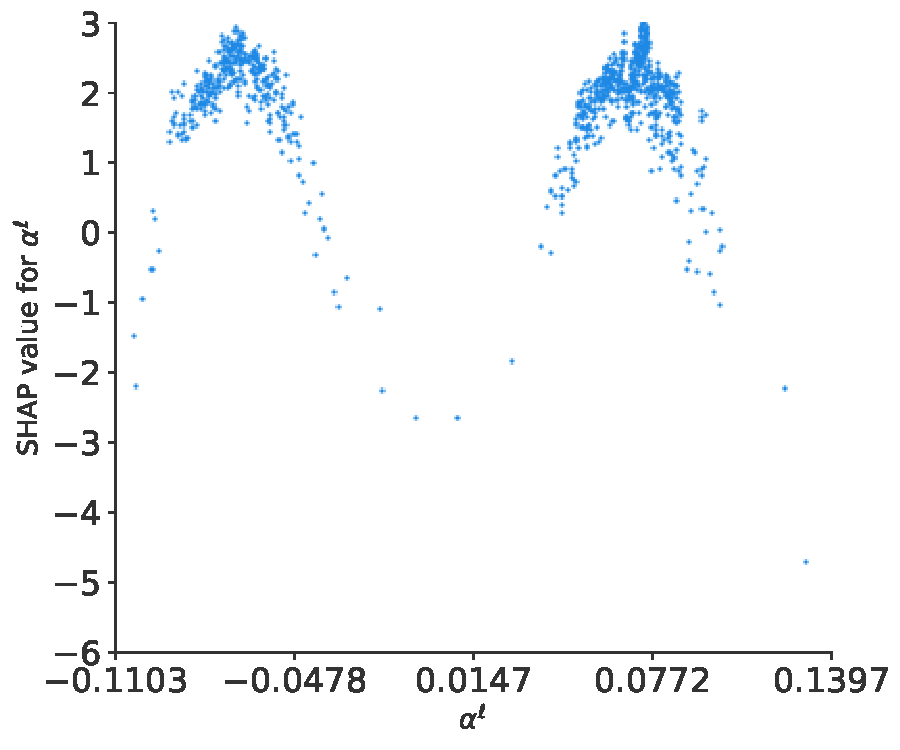
\includegraphics[width=0.30\textwidth]{figures/SHAP_al.pdf}
        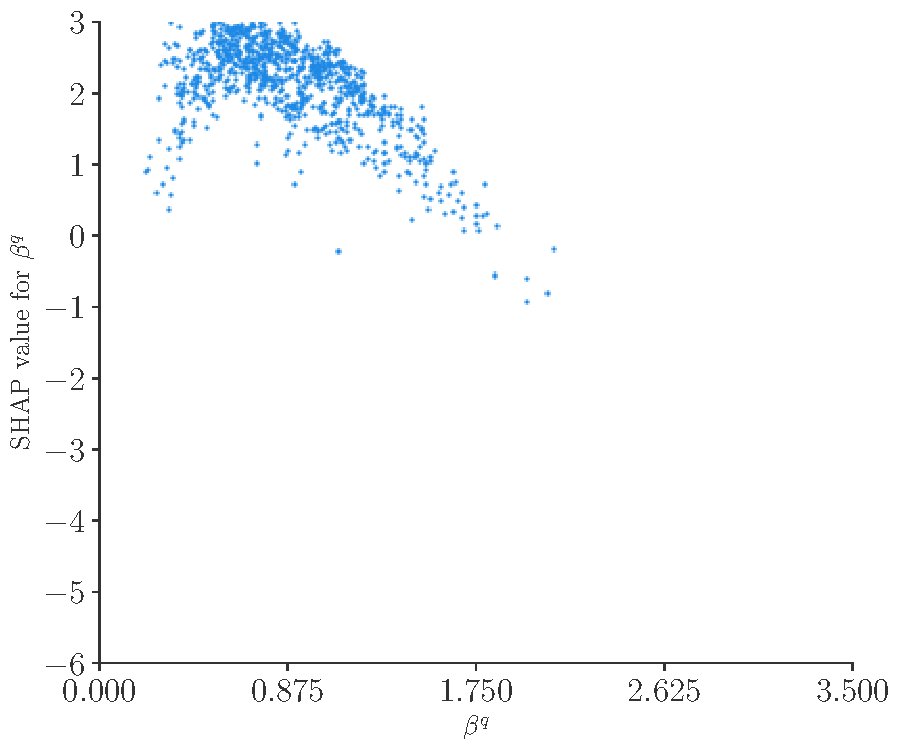
\includegraphics[width=0.30\textwidth]{figures/SHAP_bq.pdf}
    \end{center}
    \begin{itemize}
        %\item Agreement between the results obtained by the
        %      Machine Learning Montecarlo algorithm proposed and the ones
        %      obtained by following the RG equations.
        \item The SHAP values reproduce correctly the
              general features of the fit.
    \end{itemize}

\end{frame}

\begin{frame}\frametitle{Correlations between observables}
    Matrix of Pearson correlation coefficients for selected observables in the Montecarlo sample:
    \begin{columns}[onlytextwidth]
        \begin{column}{0.6\textwidth}
            \begin{tikzpicture}
                \node[anchor=south west,inner sep=0] at (0,0) {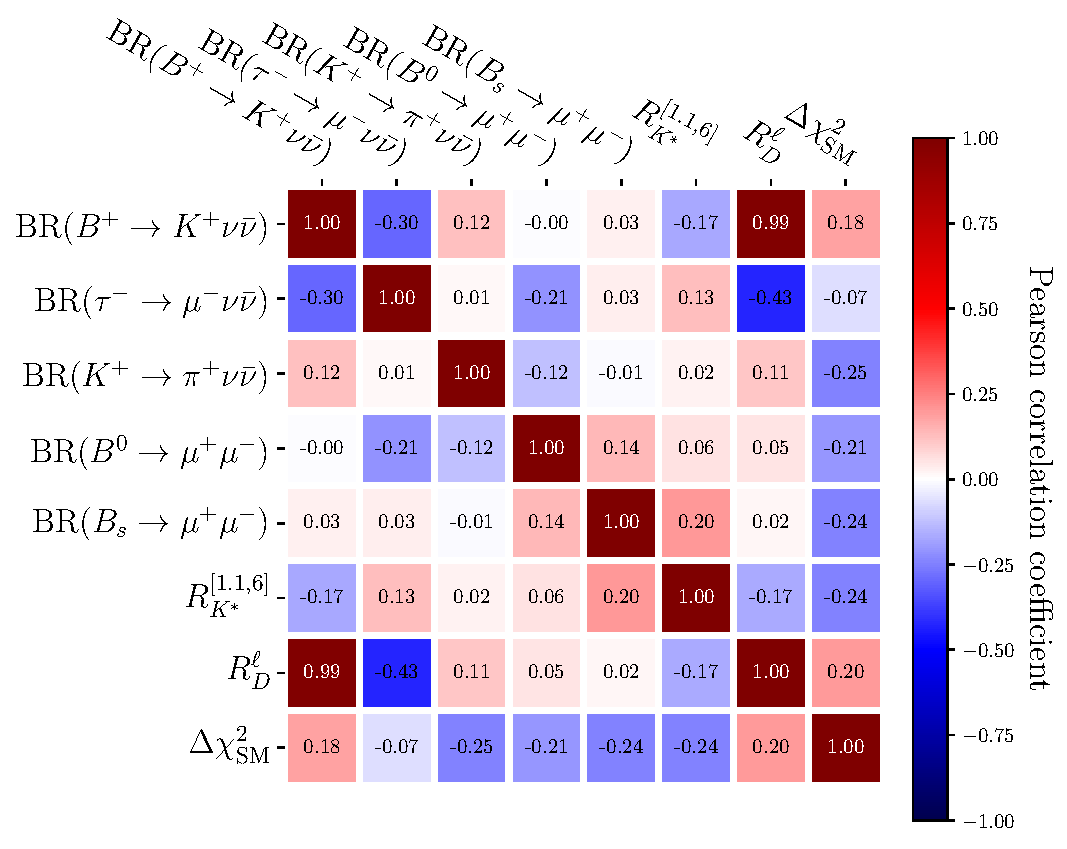
\includegraphics[width=\columnwidth]{figures/obscorr.pdf}};
                \draw[color = OliveGreen, line width=0.5mm] (1.95,1.1) circle (8pt);
                \draw[color = OliveGreen, line width=0.5mm] (4.7,3.8) circle (8pt);
            \end{tikzpicture}

        \end{column}
        \begin{column}{0.4\textwidth}
            \begin{itemize}
                \item Moderate correlation between $R_K$ and $\mathrm{BR}(B_s \to \mu^+ \mu^-)$ because $C_9^\mu \neq C_{10}^\mu$.
                \item Also moderate correlation between $R_K$ and $R_D$.
                \item {\color{OliveGreen}{Perfect correlation between} $R_D$
                      $\mathrm{BR}(B\to K^{(*)}\nu\bar{\nu})$}.
                \item No observable displays large correlations to the global likelihood: global fits are needed.
            \end{itemize}
        \end{column}
    \end{columns}

\end{frame}

\begin{frame}\frametitle{$R_D$ and $\mathrm{BR}(B\to K^{(*)}\nu\bar{\nu})$}

    \begin{center}
        \begin{columns}[onlytextwidth]
            \begin{column}{0.55\textwidth}
                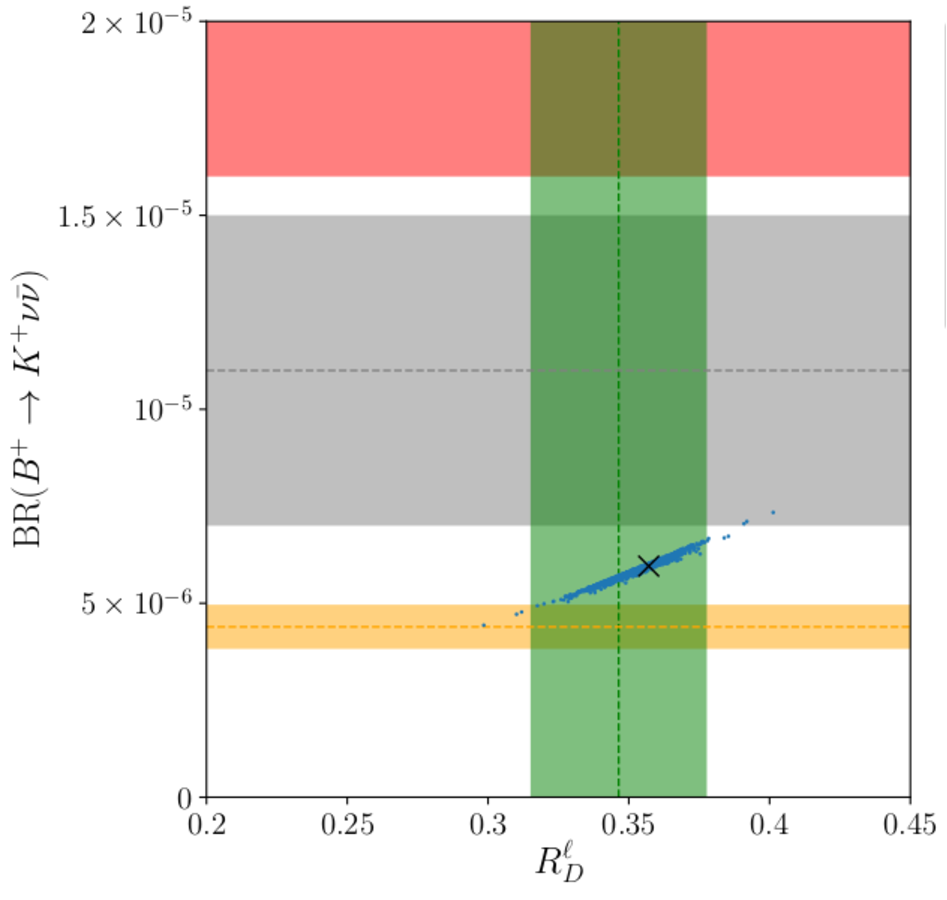
\includegraphics[width=\textwidth]{figures/RD_BKnunu_plot.pdf}
            \end{column}
            \begin{column}{0.45\textwidth}
                
\includegraphics[width=\textwidth]{figures/RD_BKnunu_leg1.pdf}\\[2pt]
                
\includegraphics[width=\textwidth]{figures/RD_BKnunu_leg2.pdf}\\[2pt]
                
\includegraphics[width=\textwidth]{figures/RD_BKnunu_leg3.pdf}\\[-6pt]
                \colorcite{Y. Ahmis \textit{et al.} (HFLAV) arXiv:1909.12524}\\[4pt]
                
\includegraphics[width=\textwidth]{figures/RD_BKnunu_leg4.pdf}\\[2pt]
                
\includegraphics[width=\textwidth]{figures/RD_BKnunu_leg5.pdf}\\[-6pt]
                \colorcite{J. Grygier \textit{et al.} (Belle) arXiv:1702.03224}\\[4pt]
                
\includegraphics[width=\textwidth]{figures/RD_BKnunu_leg6.pdf}\\[-6pt]
                \colorcite{F. Dattola (Belle-II) arXiv:2105.05754}
            \end{column}
        \end{columns}

    \end{center}

    An excess in $R_D$ implies an excess in $\mathrm{BR}(B\to K^{(*)}\nu\bar{\nu})$. \\(Note that the {\color{gray}2021 World Average} is not included in our fit).

\end{frame}

\end{document}